
\section{Experiments}\label{sect:experiments}

We start this section by detailing the benchmarks we use, the parameters of our algorithms and name our algorithm configurations for convenience. Section~\ref{sect:ftr-select} then evaluates the impact of different decision tree algorithms. Section~\ref{evaluates} the performance of \FULL and \DRAW for different configurations then compares the \FULL, \DRAW and program-based model techniques.
 
\subsection{Experimental Data, Parameters}\label{sect:data_sets}

Our investigation uses 17 symbolic regression benchmarks from~\cite{benchmarks}. All of the benchmarks are defined such that the dependent variable is the output of a particular mathematical function for a given set of inputs.  All of the inputs are taken to form a grid on some interval.  Let $E[a, b, c]$ denote $c$ samples equally spaced in the interval $[a,b]$. (Note that McDermott et al. defines $E[a, b, c]$ slightly differently.)  Below is a list of all of the benchmarks that are used:

\begin{enumerate}[noitemsep]
\item \textbf{Keijzer1}: $0.3x \sin(2 \pi x);$ $x \in E[-1,1,20]$
\item \textbf{Keijzer11}: $x y+\sin((x-1)(y-1));$ $x, y \in E[-3,3,5]$
\item \textbf{Keijzer12}: $x^{4}-x^{3}+\frac{y^{2}}{2}-y;$ $x, y \in E[-3,3,5]$
\item \textbf{Keijzer13}: $6 \sin(x) \cos(y);$ $x, y \in E[-3,3,5]$
\item \textbf{Keijzer14}: $\frac{8}{2 + x^{2} + y^{2}};$ $x,y \in E[-3,3,5]$
\item \textbf{Keijzer15}: $\frac{x^{3}}{5} - \frac{y^{3}}{2} - y - x;$ $x, y \in E[-3,3,5]$
\item \textbf{Keijzer4}: $x^{3} e^{-x} \cos(x) \sin(x) (\sin^{2}(x) \cos(x) - 1);$ $x \in E[0,10,20]$
\item \textbf{Keijzer5}: $\frac{3 x z}{(x - 10) y^{2}};$ $x,y \in E[-1,1,4]; z \in E[1,2,4]$
\item \textbf{Nguyen10}: $2 \sin(x) \cos(y);$ $x,y \in E[0,1,5]$
\item \textbf{Nguyen12}: $x^{4} - x^{3} + \frac{y^{2}}{2} - y;$ $x,y \in E[0,1,5]$
\item \textbf{Nguyen3}: $x^{5} + x^{4} + x^{3} + x^{2} + x;$ $x \in E[-1,1,20]$
\item \textbf{Nguyen4}: $x^{6} + x^{5} + x^{4} + x^{3} + x^{2} + x;$ $x \in E[-1,1,20]$
\item \textbf{Nguyen5}: $\sin(x^{2}) \cos(x) - 1;$ $x \in E[-1,1,20]$
\item \textbf{Nguyen6}: $\sin(x) + \sin(x + x^{2});$ $x \in E[-1,1,20]$
\item \textbf{Nguyen7}: $\ln(x + 1) + \ln(x^{2} + 1);$ $x \in E[0,2,20]$
\item \textbf{Nguyen9}: $\sin(x) + \sin(y^{2});$ $x,y \in E[0,1,5]$
\item \textbf{Sext}: $x^{6} - 2 x^{4} + x^{2};$ $x \in E[-1,1,20]$
\end{enumerate}

We use a standard implementation of GP from~\cite{} and chose parameters according to settings documented in~\cite{krawiecGECCO14}.
\textbf{Fixed Parameters}\label{appendix:fixed_parameters}

\begin{itemize}
\item \textbf{Tournament size}: 4
\item \textbf{Population size}: 100
\item \textbf{Number of Generations}: 250
\item \textbf{Maximum Program Tree Depth}: 17
\item \textbf{Function set}: $\{ +, -, *, /, \log, \exp, \sin, \cos, -x \}$
\item \textbf{Terminal set}: Only the features in the benchmark.
\item \textbf{Archive Capacity}: 50
\item \textbf{Mutation Rate $\mu$}: 0.1
\item \textbf{Crossover Rate with Archive configuration $\chi$}: 0.0
\item \textbf{Crossover Rate with GP $\chi$}: 0.9
\item \textbf{Archive-Based Crossover Rate $\alpha$}: 0.9
\item \textbf{REPTree}  defaults but no pruning
\item \textbf{\SCIKIT} defaults
\end{itemize}

First we replicated with 3 BGP algorithm configurations that use REPTree from KK et al's work on the symbolic regression benchmarks. These we name BGP2A, BGP4, BGP4A where the 2 indicates that no information from modeling flowed back to selection. The number 4 indicates that a program's fitness was modified by the model error $e$ and size $c$.   The suffix A indicates whether or not subprograms from the model were qualified for archive insertion and archive retrieval during BGP crossover. We observed results consistent with the prior work. Our open source software is available on GIT.

This allowed us to proceed to evaluate feature selection sensitivity based on modeling algorithm.

\subsection{Feature Selection Sensitivity}\label{sect:ftr-select}

For the algorithm configurations we adopt a clearer notation. We drop the BGP prefix and we use $M$ or $\hat M$ to designate whether model error was integrated into program fitness and $A$ of $\hat A$ to designate whether subprograms were were qualified for archive insertion and archive retrieval during BGP crossover.

Q1. Does the feature selection bias of the model step matter? 

\begin{table}[ht]
\centering
\small
\begin{tabular}{ c | c c c }
\hline\hline
& Configuration & & Average Rank \\
\hline
1 & BP2A & \REPTree & 1.82 \\
2 & BP2A & \SCIKIT  & 2.94 \\
3 & BP4A & \SCIKIT  & 3.06 \\
4 & BP4 & \SCIKIT  & 3.18 \\
5 & BP4A & \REPTree & 4.65 \\
6 & BP4 & \REPTree & 5.35 \\
\end{tabular}
\caption{Comparison of impact of \REPTree vs \SCIKIT for average fitness rank across all data sets.}
\label{table:ranksReTreeVCART}
\end{table}


Look at Table~\ref{table:ranksReTreeVCART} for rankings by fitness, averaged across the benchmark set.


\begin{table*}[ht]
\centering
%\begin{adjustbox}{width=1\textwidth}
\tiny
%\begin{tabularx}{\linewidth}{|>{\RaggedRight}p{2.5cm}|x|x|x|}\hline
\begin{tabular}{ c c c c c c c c c c c c c c c c c c c }
\hline\hline
 & & Keij1 & Keij11 & Keij12 & Keij13 & Keij14 & Keij15 & Keij4 & Keij5 & Nguy10 & Nguy12 & Nguy3 & Nguy4 & Nguy5 & Nguy6 & Nguy7 & Nguy9 & Sext \\
\hline
BP2A & \REPTree & \textbf{0.243} & 0.776 & 0.972 & \textbf{0.393} & 0.723 & \textbf{0.883} & \textbf{0.384} & \textbf{0.975} & \textbf{0.11} & \textbf{0.343} & 0.196 & \textbf{0.265} & 0.037 & 0.091 & 0.122 & 0.068 & \textbf{0.052} \\
 & \SCIKIT & 0.327 & 0.769 & \textbf{0.966} & 0.481 & 0.726 & 0.907 & 0.468 & 0.977 & 0.199 & 0.379 & 0.2 & 0.285 & 0.04 & 0.119 & 0.127 & 0.075 & 0.054 \\
BP4 & \REPTree & 0.359 & 0.852 & 0.982 & 0.817 & 0.872 & 0.922 & 0.522 & 0.993 & 0.309 & 0.388 & \textbf{0.193} & 0.33 & 0.103 & 0.133 & 0.117 & 0.165 & 0.127 \\
 & \SCIKIT & 0.357 & \textbf{0.684} & 0.968 & 0.548 & 0.776 & 0.887 & 0.513 & 0.991 & 0.144 & 0.36 & 0.266 & 0.288 & 0.126 & \textbf{0.0} & \textbf{0.104} & \textbf{0.04} & 0.083 \\
BP4A & \REPTree & 0.319 & 0.804 & 0.981 & 0.765 & 0.821 & 0.919 & 0.505 & 0.991 & 0.209 & 0.386 & 0.22 & 0.328 & 0.088 & 0.117 & 0.128 & 0.194 & 0.1 \\
 & \SCIKIT & 0.261 & 0.811 & 0.973 & 0.507 & \textbf{0.691} & 0.94 & 0.471 & 0.981 & 0.264 & 0.379 & 0.219 & 0.273 & \textbf{0.034} & 0.088 & 0.115 & 0.065 & 0.056 \\
\hline
\end{tabular}
%\end{adjustbox}
\caption{Comparison of different decision tree algorithms: \REPTREE and \SCIKIT on average program error for best of run programs (averaged across 30 runs). N.B. program error does NOT include program size. During evolution the fitness of a program integrates program error and size per\cite{krawiecGecco2014}}
\label{table:fitnessReTreeVCART}
\end{table*}


Look at Table~\ref{table:fitnessReTreeVCART} for fitness, averaged across the benchmark set.


\begin{figure}[htbp]
\begin{center}
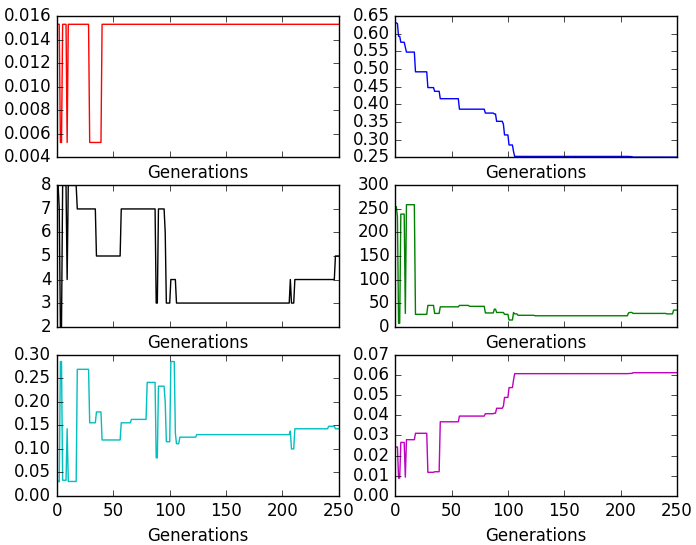
\includegraphics[width=0.99\linewidth]{sections/figures/figure_reptree.png}
\caption{We take one run of Keijzer1 running with \REPTREE modeling and configuration BP4.   We plot on the first row  model error on the left and the fitness of the best program (right).  The plots on the second row show number of features of model  and number of subprograms in the best program (right). The plots on the third row show the ratio of number of model features to program subtrees (left) and ratio of model error to program fitness. Since the run is configured for  BP4 program fitness integrates both model error and complexity.}
\label{fig:deepdive}
\end{center}
\end{figure}


Describe difference in implementations between Reptree and SKL-RepTree.\\
Need REPTREE and Scikit learn algorithm references and links to their code.

Compare REPTREE TO SICKIT LEARN for BGP 2A, 4a, 4 getting 6 combinations\\
Reference Table~\ref{table:avg_fitness} comparing average program error among BGP2A, BGP4, BGP4A, GP for 17 functions with REPTREE and ScikitLearn implementation.\\
Reference Table~\ref{table:avg_size} showing average program size among BGP2A, BGP4, BGP4A, GP for 17 functions with REPTREE and ScikitLearn implementation.\\
STDEV is in separate table in thesis, how to handle in paper?

Statistical testing required!!

Include a ranking table.  just on error of program and only 6 combinations (two choices of decision tree implementation) and 3 algorithms (2A,4,4A). 

Select 1 run, 1 dataset: what is \# of features in model of best individual at first and final generation (each generation)? What is fraction of \# of features in model to \# of subtrees in best individual at first and final generation (each generation)?  (Each generation) means we would have a plot (fitness on Y1 axis, features/fraction on Y2, Y3 and X is generations). We could amass these statistics for every dataset and 30 runs but lower priority than other tasks.

Segue to next subsection: Do features depend on one another? We're identifying their model value in the context of the same tree. They could be co-adapted and not very good with any other tree. We investigate further.

\subsection{Aggregate Trace Matrices}\label{sect:agg-features}


\begin{table*}[ht]
\centering
%\begin{adjustbox}{width=1\textwidth}
\small
\begin{tabular}{ c | c c c ||  c c c c }
 $C$& $\hat M A$ & $M \hat A$ & $MA$ & $\hat M A$ & $M \hat A$ & $MA$\\ \hline
 25 & 3.06 & 2.24 & 2.35 & \textbf{1.65} & 2.18 & \textbf{1.41} \\
 50 & \textbf{2.29} & \textbf{1.82} & \textbf{1.88} & 2.41 & \textbf{1.88} & 2.29 \\
 75 & \textbf{2.29} & 2.0 & 2.0 & 3.06 & 2.12 & 2.65 \\
 100 & 2.35 & 3.94 & 3.76 &2.88 & 3.82 & 3.65  \\
%\hline
\end{tabular}
%\end{adjustbox}
\caption{\DRAW (lhs) and \FULL (rhs) average rank varying model fitness signal (M or $\hat M$) and use of archive (A or $\hat A$) for 17 benchmarks}
\label{table:XXdraws_avg_ranks}
\end{table*}


%\input{sections/fullpop_average_ranks}

And here is the average fitness table ....

\begin{table*}[ht]
\tiny
\centering
%\begin{adjustbox}{width=1\textwidth}
\begin{tabular}{ c | c | c c c c c c c c c c c c c c c c c }
%\hline\hline
 & & Keij1 & Keij11 & Keij12 & Keij13 & Keij14 & Keij15 & Keij4 & Keij5 & Nguy10 & Nguy12 & Nguy3 & Nguy4 & Nguy5 & Nguy6 & Nguy7 & Nguy9 & Sext \\
 \hline
& Draw 25 & 0.306 & 0.704 & 0.976 & 0.436 & 0.768 & \textbf{0.845} & 0.371 & 0.975 & 0.162 & 0.341 & \textbf{0.172} & 0.301 & 0.056 & 0.074 & 0.132 & 0.241 & 0.058 \\
$\bar M A$ & Draw 50 & 0.286 & \textbf{0.604} & 0.969 & 0.422 & 0.731 & 0.866 & 0.376 & \textbf{0.967} & 0.107 & 0.353 & 0.194 & 0.295 & 0.045 & 0.089 & \textbf{0.103} & 0.159 & 0.059 \\
 & Draw 75 & \textbf{0.246} & 0.716 & 0.968 & \textbf{0.325} & 0.736 & 0.869 & 0.347 & 0.974 & \textbf{0.089} & 0.351 & 0.215 & 0.278 & 0.06 & 0.1 & 0.118 & 0.206 & \textbf{0.044} \\
 & Draw 100 & 0.253 & 0.695 & 0.969 & 0.382 & \textbf{0.716} & 0.877 & \textbf{0.33} & 0.972 & 0.123 & 0.356 & 0.217 & 0.285 & \textbf{0.03} & 0.129 & 0.115 & 0.165 & 0.047 \\
 \hline
 & Full 25 & 0.278 & 0.812 & \textbf{0.956} & 0.621 & 0.761 & 0.88 & 0.457 & 0.977 & 0.232 & 0.385 & 0.297 & 0.33 & 0.058 & 0.159 & 0.204 & 0.212 & 0.062 \\
 & Full 50 & 0.279 & 0.883 & 0.979 & 0.564 & 0.748 & 0.921 & 0.411 & 0.981 & 0.294 & 0.387 & 0.337 & 0.37 & 0.06 & 0.264 & 0.195 & 0.301 & 0.086 \\
 & Full 75 & 0.302 & 0.864 & 0.976 & 0.604 & 0.804 & 0.925 & 0.453 & 0.982 & 0.364 & 0.395 & 0.316 & 0.361 & 0.059 & 0.271 & 0.225 & 0.306 & 0.088 \\
 & Full 100 & 0.272 & 0.864 & 0.982 & 0.565 & 0.809 & 0.947 & 0.397 & 0.977 & 0.304 & 0.393 & 0.376 & 0.372 & 0.081 & 0.277 & 0.179 & 0.214 & 0.129 \\
 \hline
& Draw 25 & 0.322 & 0.89 & 0.979 & 0.732 & 0.786 & 0.889 & 0.601 & 0.991 & 0.185 & 0.361 & 0.233 & 0.283 & 0.107 & 0.103 & 0.144 & 0.197 & 0.076 \\
$M \bar A$ & Draw 50 & 0.314 & 0.824 & 0.979 & 0.697 & 0.798 & 0.888 & 0.55 & 0.986 & 0.183 & 0.393 & 0.307 & 0.322 & 0.081 & 0.088 & 0.15 & 0.165 & 0.081 \\
 & Draw 75 & 0.337 & 0.865 & 0.979 & 0.723 & 0.819 & 0.886 & 0.562 & 0.99 & 0.22 & 0.356 & 0.236 & 0.246 & 0.064 & 0.108 & 0.136 & 0.242 & 0.088 \\
 & Draw 100 & 0.367 & 0.908 & 0.986 & 0.879 & 0.846 & 0.962 & 0.598 & 0.993 & 0.377 & 0.43 & 0.363 & 0.442 & 0.156 & 0.186 & 0.246 & 0.267 & 0.127 \\
 \hline
 & Full 25 & 0.288 & 0.875 & 0.973 & 0.478 & 0.783 & 0.867 & 0.516 & 0.987 & 0.163 & 0.346 & 0.23 & 0.302 & 0.072 & \textbf{0.069} & 0.119 & 0.174 & 0.093 \\
 & Full 50 & 0.301 & 0.851 & 0.967 & 0.463 & 0.834 & 0.894 & 0.52 & 0.984 & 0.121 & \textbf{0.338} & 0.23 & 0.274 & 0.048 & 0.117 & 0.144 & \textbf{0.132} & 0.066 \\
 & Full 75 & 0.317 & 0.824 & 0.974 & 0.538 & 0.781 & 0.886 & 0.499 & 0.986 & 0.168 & 0.353 & 0.188 & \textbf{0.23} & 0.067 & 0.085 & 0.161 & 0.172 & 0.074 \\
 & Full 100 & 0.368 & 0.833 & 0.979 & 0.708 & 0.838 & 0.949 & 0.536 & 0.991 & 0.218 & 0.384 & 0.321 & 0.318 & 0.083 & 0.198 & 0.157 & 0.24 & 0.129 \\
 \hline
& Draw 25 & 0.301 & 0.808 & 0.976 & 0.625 & 0.798 & 0.919 & 0.385 & 0.984 & 0.211 & 0.361 & 0.287 & 0.329 & 0.082 & 0.205 & 0.147 & 0.336 & 0.072 \\
$M A$ & Draw 50 & 0.295 & 0.803 & 0.975 & 0.54 & 0.735 & 0.927 & 0.404 & 0.984 & 0.235 & 0.349 & 0.303 & 0.296 & 0.073 & 0.204 & 0.156 & 0.287 & 0.074 \\
 & Draw 75 & 0.292 & 0.797 & 0.975 & 0.567 & 0.73 & 0.937 & 0.426 & 0.988 & 0.274 & 0.364 & 0.257 & 0.329 & 0.06 & 0.171 & 0.124 & 0.318 & 0.074 \\
 & Draw 100 & 0.306 & 0.866 & 0.986 & 0.814 & 0.751 & 0.961 & 0.489 & 0.991 & 0.315 & 0.408 & 0.393 & 0.455 & 0.113 & 0.255 & 0.24 & 0.257 & 0.093 \\
 \hline
 & Full 25 & 0.304 & 0.847 & 0.974 & 0.685 & 0.767 & 0.936 & 0.498 & 0.985 & 0.282 & 0.358 & 0.295 & 0.384 & 0.067 & 0.262 & 0.188 & 0.271 & 0.086 \\
 & Full 50 & 0.315 & 0.872 & 0.981 & 0.656 & 0.763 & 0.936 & 0.421 & 0.988 & 0.349 & 0.369 & 0.356 & 0.452 & 0.072 & 0.302 & 0.271 & 0.289 & 0.098 \\
 & Full 75 & 0.317 & 0.902 & 0.984 & 0.626 & 0.78 & 0.95 & 0.474 & 0.986 & 0.326 & 0.394 & 0.397 & 0.436 & 0.097 & 0.351 & 0.239 & 0.357 & 0.13 \\
 & Full 100 & 0.326 & 0.903 & 0.987 & 0.759 & 0.81 & 0.953 & 0.496 & 0.989 & 0.428 & 0.423 & 0.507 & 0.449 & 0.158 & 0.383 & 0.268 & 0.236 & 0.168 \\
\end{tabular}
%\end{adjustbox}
\caption{Average fitness of each configuration across all data sets.}
\label{table:ranks}
\end{table*}


\begin{table*}[ht]
\centering
%\begin{adjustbox}{width=1\textwidth}
\tiny
\begin{tabular}{ c | c  |c c c c c c c c c c c c c c c c c }
%\hline\hline
 & & Keij1 & Keij11 & Keij12 & Keij13 & Keij14 & Keij15 & Keij4 & Keij5 & Nguy10 & Nguy12 & Nguy3 & Nguy4 & Nguy5 & Nguy6 & Nguy7 & Nguy9 & Sext \\
\hline
 & Draw 25 & 4 & 3 & 4 & 4 & 4 & 1 & 3 & 4 & 4 & 1 & 1 & 4 & 3 & 1 & 4 & 4 & 3 \\
$\bar M A$ & Draw 50 & 3 & 1 & 3 & 3 & 2 & 2 & 4 & 1 & 2 & 3 & 2 & 3 & 2 & 2 & 1 & 1 & 4 \\
 & Draw 75 & 1 & 4 & 1 & 1 & 3 & 3 & 2 & 3 & 1 & 2 & 3 & 1 & 4 & 3 & 3 & 3 & 1 \\
 & Draw 100 & 2 & 2 & 2 & 2 & 1 & 4 & 1 & 2 & 3 & 4 & 4 & 2 & 1 & 4 & 2 & 2 & 2 \\
 \hline
 & Full 25 & 2 & 1 & 1 & 4 & 2 & 1 & 4 & 2 & 1 & 1 & 1 & 1 & 1 & 1 & 3 & 1 & 1 \\
 & Full 50 & 3 & 4 & 3 & 1 & 1 & 2 & 2 & 3 & 2 & 2 & 3 & 3 & 3 & 2 & 2 & 3 & 2 \\
 & Full 75 & 4 & 2 & 2 & 3 & 3 & 3 & 3 & 4 & 4 & 4 & 2 & 2 & 2 & 3 & 4 & 4 & 3 \\
 & Full 100 & 1 & 3 & 4 & 2 & 4 & 4 & 1 & 1 & 3 & 3 & 4 & 4 & 4 & 4 & 1 & 2 & 4 \\
 \hline
 & Draw 25 & 2 & 3 & 2 & 3 & 1 & 3 & 4 & 3 & 2 & 2 & 1 & 2 & 3 & 2 & 2 & 2 & 1 \\
$M \bar A$ & Draw 50 & 1 & 1 & 3 & 1 & 2 & 2 & 1 & 1 & 1 & 3 & 3 & 3 & 2 & 1 & 3 & 1 & 2 \\
 & Draw 75 & 3 & 2 & 1 & 2 & 3 & 1 & 2 & 2 & 3 & 1 & 2 & 1 & 1 & 3 & 1 & 3 & 3 \\
 & Draw 100 & 4 & 4 & 4 & 4 & 4 & 4 & 3 & 4 & 4 & 4 & 4 & 4 & 4 & 4 & 4 & 4 & 4 \\
 \hline
 & Full 25 & 1 & 4 & 2 & 2 & 2 & 1 & 2 & 3 & 2 & 2 & 2 & 3 & 3 & 1 & 1 & 3 & 3 \\
 & Full 50 & 2 & 3 & 1 & 1 & 3 & 3 & 3 & 1 & 1 & 1 & 3 & 2 & 1 & 3 & 2 & 1 & 1 \\
 & Full 75 & 3 & 1 & 3 & 3 & 1 & 2 & 1 & 2 & 3 & 3 & 1 & 1 & 2 & 2 & 4 & 2 & 2 \\
 & Full 100 & 4 & 2 & 4 & 4 & 4 & 4 & 4 & 4 & 4 & 4 & 4 & 4 & 4 & 4 & 3 & 4 & 4 \\
 \hline
& Draw 25 & 3 & 3 & 3 & 3 & 4 & 1 & 1 & 2 & 1 & 2 & 2 & 2 & 3 & 3 & 2 & 4 & 1 \\
$M A$  & Draw 50 & 2 & 2 & 1 & 1 & 2 & 2 & 2 & 1 & 2 & 1 & 3 & 1 & 2 & 2 & 3 & 2 & 3 \\
 & Draw 75 & 1 & 1 & 2 & 2 & 1 & 3 & 3 & 3 & 3 & 3 & 1 & 3 & 1 & 1 & 1 & 3 & 2 \\
 & Draw 100 & 4 & 4 & 4 & 4 & 3 & 4 & 4 & 4 & 4 & 4 & 4 & 4 & 4 & 4 & 4 & 1 & 4 \\
 \hline
 & Full 25 & 1 & 1 & 1 & 3 & 2 & 1 & 4 & 1 & 1 & 1 & 1 & 1 & 1 & 1 & 1 & 2 & 1 \\
 & Full 50 & 2 & 2 & 2 & 2 & 1 & 2 & 1 & 3 & 3 & 2 & 2 & 4 & 2 & 2 & 4 & 3 & 2 \\
 & Full 75 & 3 & 3 & 3 & 1 & 3 & 3 & 2 & 2 & 2 & 3 & 3 & 2 & 3 & 3 & 2 & 4 & 3 \\
 & Full 100 & 4 & 4 & 4 & 4 & 4 & 4 & 3 & 4 & 4 & 4 & 4 & 3 & 4 & 4 & 3 & 1 & 4 \\
%\hline
\end{tabular}
%\end{adjustbox}
\caption{Rank based program error for best of run programs.}
\label{table:rank_program_error_draw_full}
\end{table*}


The question is what aggregations? What if we take everyone?

show discuss results of full-pop (call it 100\_XX)\\

Detailed study: take 1 run, 1 dataset (save seed!) and one algorithm of 2A,3,3A and one choice of decision tree.  What dataset? Choices: use hardest problem, or one that 2A,3,3A don't do as well as GP on. \\
How many programs have one or more features in the model?\\ how many programs have 2, 3, etc? This says something about co-adaptation. Were pairs of features subtrees where one was within the other?  \\what is the ratio of model features to total-features-in-pop? \\how many features are in the model (first, final generations?) (maybe plot every generation ( very low priority))

Now what if we discriminate the aggregation set by fitness so we're only identifying features from superior parts of the population?

We create 3 additional  aggregate trace matrices: 25, 50, 75,  where pop is sorted low to high by fitness (error + size) and then cut off at these different thresholds. 

Show/describe a longitudinal comparison of all 4 and add in best of program-trace resutls.

Does the discrimination by program fitness plus the aggregation among programs work better than just program trace? SHOW GRAND RANKING.

%\TODO{Insert my sketch of tables of results}
%
%\TODO{Not for Monday night but if we get accepted, we can increase the number of runs and robustness of the detailed results to encompass more datasets or more runs and provide average and standard deviation}
